\documentclass{jsarticle}

\usepackage{url}
\usepackage[dvipdfmx]{graphicx}

\title{VideoCore IV の概要と性能}
\author{杉崎 行優}

\begin{document}

\maketitle{}
\abstract{
Raspberry Pi 1 の SoC である BCM2835、また、
Raspberry Pi 2 の SoC である BCM2836 には、VideoCore IV という、
GPU の役割を果たすプロセッサが組み込まれている。
本記事では文献を参考にし、VideoCore IV の概要を記す。
また、実際にプログラムを書き、VideoCore IV の性能を測定する。
}
\tableofcontents
\newpage

\section{はじめに}

\subsection{本記事における用語と略称}

本記事における用語は一般的に用いられているものを用いる。
また、本記事においては BCM2835 と BCM2836 を「本対象 SoC」と記す。

\subsection{Broadcom Corporation による VideoCore IV の情報や
ライブラリの公開}

VideoCore IV プロセッサを開発し、それを含む製品を販売している
Broadcom Corporation は2014年2月28日、Raspberry Pi が初めて発表されてから
2年が経過した記念として ``VideoCore IV Architecture Reference Guide'' を
公開した。これは VideoCore IV のシステムや命令等の仕様を詳細に記した
ドキュメントである。また、Broadcom Corporation は同時に
EGL、OpenGL、OpenGL ES、OpenVG、OpenMAX といった
グラフィック・オーディオライブラリを本対象 SoC 向けに移植したコードと、
VideoCore IV のリアルタイム OS のコードを公開した。

\subsection{特許 US20110264902}

アメリカ合衆国で取得された特許
``METHOD AND SYSTEM FOR SUSPENDING VIDEO PROCESSOR AND SAVING PROCESSOR
STATE IN SDRAM UTILIZING A CORE PROCESSOR" \cite{vc-patent} に、
アンテナやキーパッドが含まれている点を除き、本対象 SoC と酷似している
SoC レイアウトの図が複数示されている。それらを図 \ref{pic:vc-fig1a}、
図 \ref{pic:vc-fig1b}、図 \ref{pic:vc-fig2}に示す。
この特許の申請主は Gordon Hollingworth という人物で、この方は
Raspberry Pi のソフトウェア開発の主導者である \cite{gh-1} \cite{gh-2}
\cite{gh-3} \cite{gh-4} \cite{gh-5} \cite{gh-6}。
以上のことから、本記事ではこの特許の SoC レイアウトの一部を
本対象 SoC のレイアウトと仮定し、参考にする。

\begin{figure}
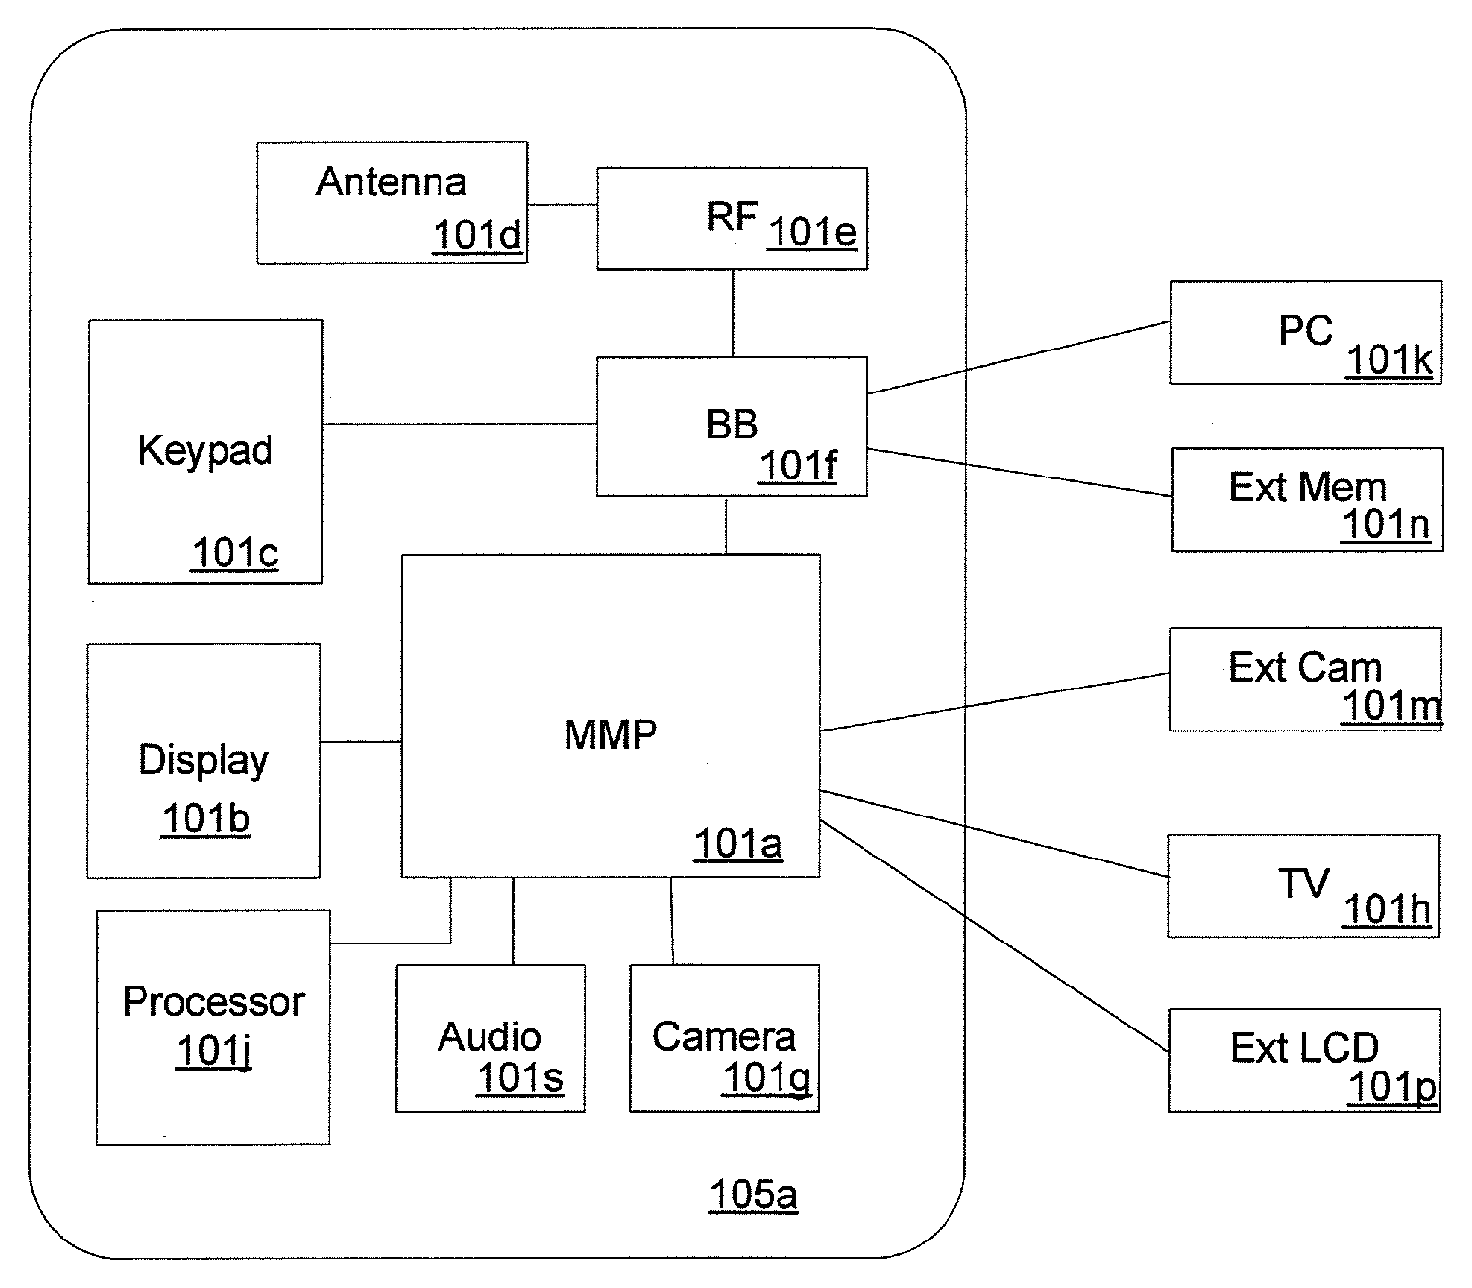
\includegraphics[width=\textwidth]{vc-fig1a.png}
\caption{文献\cite{vc-patent}から引用した図 1}
\label{pic:vc-fig1a}
\end{figure}

\begin{figure}
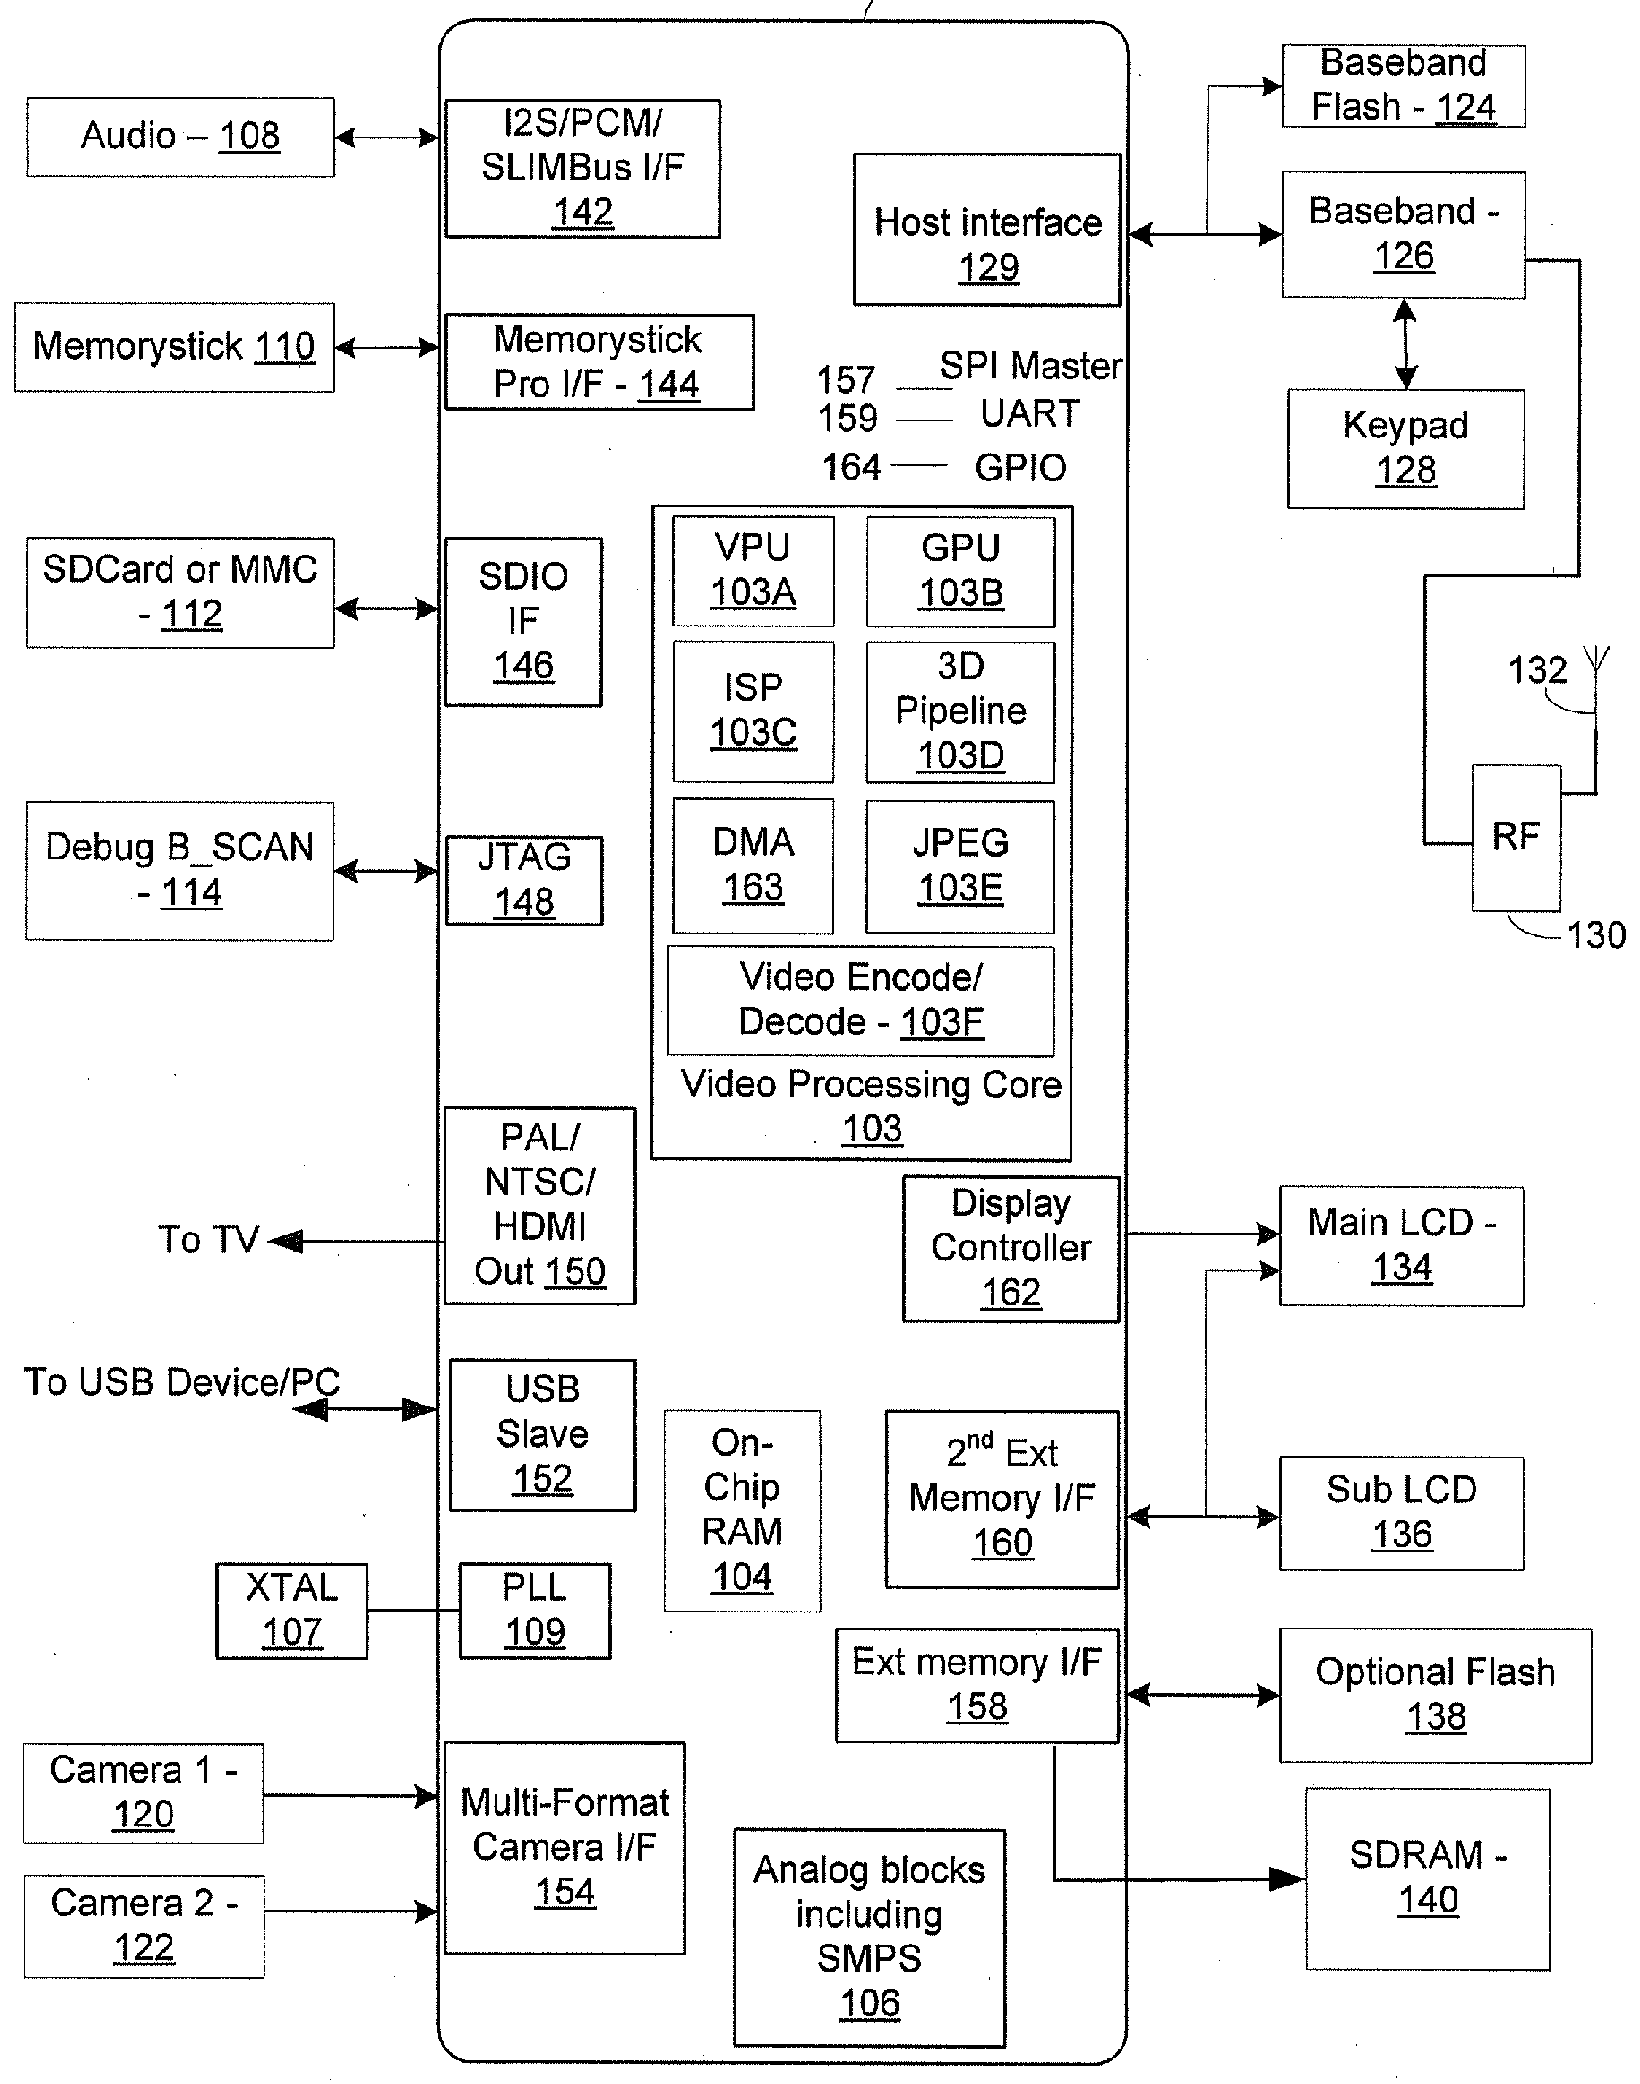
\includegraphics[width=\textwidth]{vc-fig1b.png}
\caption{文献\cite{vc-patent}から引用した図 2}
\label{pic:vc-fig1b}
\end{figure}

\begin{figure}
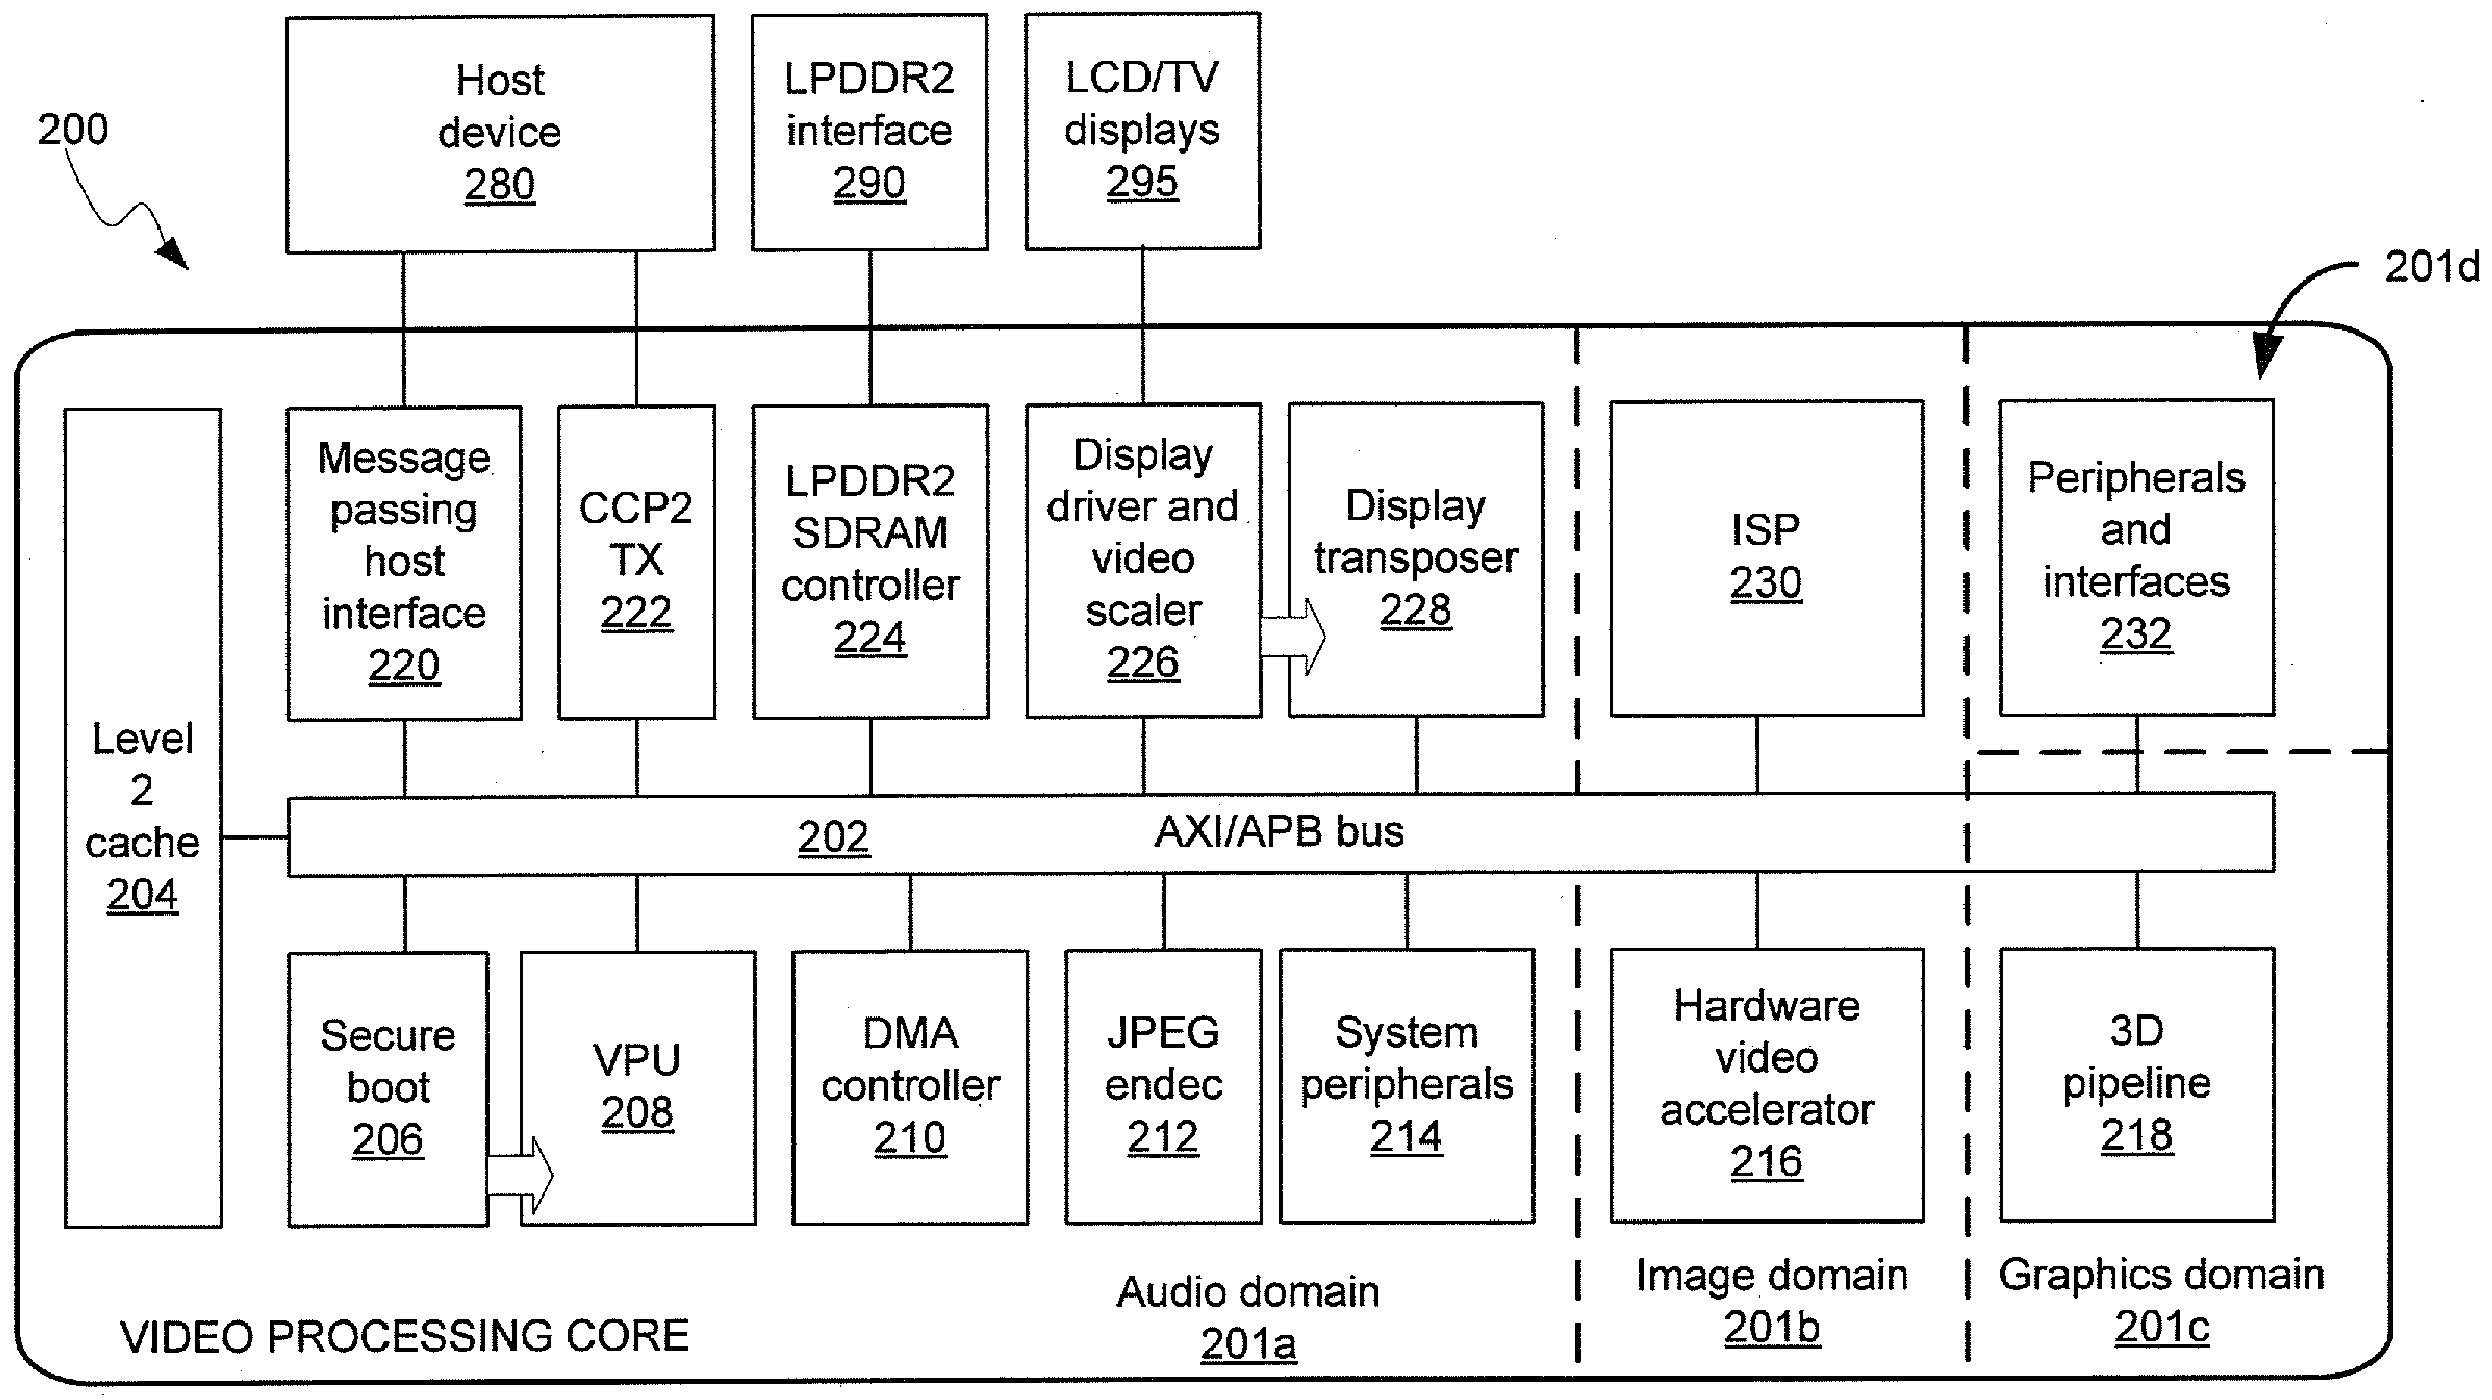
\includegraphics[width=\textwidth]{vc-fig2.png}
\caption{文献\cite{vc-patent}から引用した図 3}
\label{pic:vc-fig2}
\end{figure}


\section{VideoCore IV の概要}

\subsection{本対象 SoC における VideoCore IV の物理的位置}

図 \ref{pic:vc-fig1a} は本対象 SoC を最も俯瞰的に見たレイアウトであると
考えられる。この図に記されている MMP は ``multimedia processor'' の意であり、
ビデオやオーディオのストリームを処理したり、各モジュールの電力管理をしたり、
外部のメモリやディスプレイ等のペリフェラルと通信するプロセッサである。
図 \ref{pic:vc-fig1b} は MMP のレイアウトである。
この図に記されている Video Processing Core のレイアウトを示したのが
図 \ref{pic:vc-fig2} である。この図より、Video Processing Core は
Level 2 cache、Secure boot、DMA controller、JPEG encoder/decoder、
Hardware video accelerator、3D pipeline 等のためのモジュールを持ち、
それぞれが AXI バスに接続されているという構造になっていることが分かる。

ここで、文献で示されている VideoCore IV のレイアウトを
図 \ref{pic:vc-vc} に示す。ここでは VideoCore IV は
VideoCore IV 3D System と呼ばれている。また、図より VideoCore IV は
AXI バスに接続された Level 2 cache 等の複数のモジュールから成ることが分かる。

以上のことから、VideoCore IV は本対象 SoC の MMP 内の
Video Processing Core 内で AXI バスに接続された、少なくとも
3D pipeline と Level 2 cache から成るシステムであることが分かる。


\bibliographystyle{unsrt}
\bibliography{refer}

\end{document}
